\documentclass[conference]{IEEEtran}
\IEEEoverridecommandlockouts
% The preceding line is only needed to identify funding in the first footnote. If that is unneeded, please comment it out.
\usepackage{cite}
\usepackage{amsmath,amssymb,amsfonts}
\usepackage{algorithmic}
\usepackage{graphicx}
\graphicspath{{./figures/}}
\usepackage{textcomp}

\usepackage[table,xcdraw]{xcolor}
\usepackage[utf8]{inputenc}
\usepackage[T1]{fontenc}
\usepackage[english]{babel}
\usepackage{microtype} % optional, for aesthetics
\usepackage{tabularx} % nice to have
\usepackage{booktabs} % necessary for style
\usepackage{graphicx}
\graphicspath{{./figures/}}
\usepackage{listings}
\usepackage{multirow}
\usepackage{hhline}
\usepackage{caption}
\usepackage{makecell}
\usepackage{ragged2e}
\usepackage{parskip}
\usepackage{wrapfig}
\usepackage{array}
\usepackage{float}
\usepackage{lipsum}
\usepackage{subcaption}
\usepackage[linesnumbered,ruled]{algorithm2e}
\usepackage{courier}
\usepackage{hyperref}
\hypersetup{colorlinks=true,allcolors=blue}
\usepackage{listings}
\usepackage{float}
\lstset{
    basicstyle=\ttfamily,
    frame=none, 
    breaklines=true,
    numbers=left,
    xleftmargin=1.5em,
    framexleftmargin=0em,
    emphstyle=\textbf,
    float=t
}
\lstdefinestyle{ocl}{
    emph={
        context, inv
    }
}
\lstdefinestyle{cbp}{
    basicstyle=\ttfamily\scriptsize,
    emph={
        session, create, type,
        set, to, add, hire
    }
}
\lstdefinestyle{xmi}{
    basicstyle=\ttfamily\scriptsize,
    emph={
        Node, children
    }
}
\lstdefinestyle{xml}{
    basicstyle=\ttfamily\scriptsize,
    emph={
        register, create, add, to, resource, at,
        from, eattribute, remove, ereference,
        set, unset, session, Roy, Jen,
        Moss, Richmond
    }
}
\lstdefinestyle{java}{
    basicstyle=\ttfamily\scriptsize,
    emph={
        case, $unset$,
        instanceof, else, if, void,
        new, UnsetEAttributeEvent,
        UnsetEReferenceEvent,
        @override, public, class, extends
    }
}
\lstdefinestyle{eol}{
    basicstyle=\ttfamily\scriptsize,
    emph={
        var, new, for, in, create, set, with, type, at,
        unset, to, add, remove, delete, register, move,
        from, position, from, move-within, session, comp, composite, \.
    }
}


\def\BibTeX{{\rm B\kern-.05em{\sc i\kern-.025em b}\kern-.08em
    T\kern-.1667em\lower.7ex\hbox{E}\kern-.125emX}}


\begin{document}

\title{Towards Visualisation of Model Construction
%    *\\
%{\footnotesize \textsuperscript{*}Note: Sub-titles are not captured in Xplore and should not be used}
%\thanks{Identify applicable funding agency here. If none, delete this.}
}

\author{
    \IEEEauthorblockN{Alfa Yohannis\IEEEauthorrefmark{1}\IEEEauthorrefmark{3}, Horacio Hoyos Rodriguez\IEEEauthorrefmark{1}, Fiona Polack\IEEEauthorrefmark{2}, Dimitris Kolovos\IEEEauthorrefmark{1}}
    \IEEEauthorblockA{\IEEEauthorrefmark{1}Department of Computer Science, University of York
        \\alfa.yohannis@merahputih.id, horacio\_hoyos\_rodriguez@ieee.org, dimitris.kolovos@york.ac.uk}
    \IEEEauthorblockA{\IEEEauthorrefmark{2}School of Computing and Maths, Keele University, United Kingdom
        \\f.a.c.polack@keele.ac.uk}
    \IEEEauthorblockA{\IEEEauthorrefmark{3}Department of Computer Science, Kalbis Institute, Indonesia}
}
\maketitle

\begin{abstract}


\end{abstract}

\begin{IEEEkeywords}
visualization, change-based persistence, model evolution, BPMN2, model-driven engineering
\end{IEEEkeywords}

\section{Introduction}
\label{sec:introduction}
In the context of model-driven engineering, models that are under-construction or completely developed are commonly persisted 
so that the construction of the models can be continued or the models can be reused for other purposes. 
Generally, these models are persisted in state-based format that is persisting their snapshots at certain points of time. 
This approach causes the models losing the details of their historical changes which are substantial resources when 
we want to perform analytical study of model evolution. As an alternative, models can also be persisted in change-based format -- models are 
persisted on their changes. This type of persistence preserves all changes applied to models.

In this paper, we extends our previous work on change-based persistence (CBP) that complies to the MOF/EMF metamodelling architectures
\cite{DBLP:conf/models/YohannisKP17,yohannis2018towards,DBLP:conf/models/YohannisRPK18,yohannis2018efficient}
by showing that a change-based persistence file can also be used as a resource to visualise changes that have been applied to construct a model. 
Our tool takes a CBP file of a model as an input and presents the persisted changes as an animated graphical model. 

This paper is structured as follows. 
Section \ref{sec:change-based_persistence} provides an overview of our previous work on change-based model persistence. 
Section \ref{sec:visualising_model_construction} discusses our approach in using change-based persistence to visualise model construction. 
Section \ref{sec:evaluation} presents the evaluation to our approach. 
Section \ref{sec:related_work} provides an overview of related work, and
Section \ref{sec:conclusions_and_future_work} concludes with a discussion on directions for future work.



\section{Change-based Persistence}
\label{sec:change-based_persistence}

Instead of persisting the snapshots of models as commonly practised in model-driven engineering, change-based model persistence persists models on their changes. 
This means that all changes applied to a model are recorded so that they can be re-used for other purposes. 

\begin{figure}[h]
    \centering
    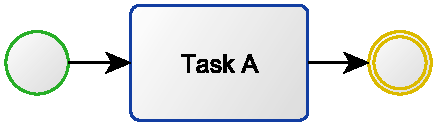
\includegraphics[width=0.5\linewidth]{bpmn2}
    \caption{A simple BPMN2 model.}
    \label{fig:bpmn2}
\end{figure}

Let's say that Bob developed a simple BPMN2 model in Fig. \ref{fig:bpmn2}. In common practice, if the model is persisted in state-based format, 
the persistence produces an XMI file (simplified) as in Lst. \ref{lst:bpmn2_xmi}. This type of persistence only preserves the eventual state of the model,  
loosing the detailed information of changes executed by Bob to construct the model. In contrary, 
if we record all the changes made by Bob and persist them into a CBP file, we might obtain a list of change events in Lst. \ref{lst:bpmn2_cbp}. 

\vspace{-15pt}
\begin{lstlisting}[style=eol,numbersep=1pt,caption={A BPMN2 model in Fig. \ref{fig:bpmn2} persisted in simplified XMI.},label=lst:bpmn2_xmi]
<process id="e1" name="Default Process">
 <startEvent id="e2" name="Start Event 1">
   <outgoing>e15</outgoing>
 </startEvent>
 <endEvent id="e4" name="End Event 1">
   <incoming>e16</incoming>
 </endEvent>
 <task id="e14" name="Task A">
   <incoming>e15</incoming>
   <outgoing>e16</outgoing>
 </task>
 <sequenceFlow id="e15" sourceRef="e2" targetRef="e14"/>
 <sequenceFlow id="e16" sourceRef="e14" targetRef="e4"/>
</process>
\end{lstlisting}


From the list, we can know the sequence of changes made by Bob to construct the model. We can also identify that Bob made invalid changes 
that connect SequenceFlow \texttt{e3} from EndEvent \texttt{e4} to StartEvent \texttt{e2}
-- no SequenceFlow is allowed to come out from an EndEvent or enter a StartEvent -- which he deleted later in the following changes. 
Such phenomenon might not be identified if we persists the model in state-based format. 

\vspace{-15pt}
\begin{lstlisting}[style=eol,numbersep=5pt,caption={The pseudo-formatted CBP of the model in Fig. \ref{fig:bpmn2}.},label=lst:bpmn2_cbp]
create e1 type Process
set e1.name to "Process 1"
create e2 type StartEvent
add e2 to e1.flowElements at 0
create e3 type SequenceFlow
set e3.name from to "Sequence Flow 1"
add e3 to e1.flowElements at 1
create e4 type EndEvent
add e4 to e1.flowElements at 0
add e3 to e2.incoming at 0
add e3 to e4.outgoing at 0
add e1 to resource at 0
remove e3 from e2.outgoing at 0 composite c1
remove e3 from e4.incoming at 0 composite c1
unset e3.name from "Sequence Flow 1" to null composite c1
remove e3 from e1.flowElements at 1 composite c1
delete e3 type SequenceFlow composite c1
create e5 type Task
set e5.name from to "Task 1"
add e5 to e1.flowElements at 2
create e6 type SequenceFlow
add e6 to e2.outgoing at 0
add e6 to e5.incoming at 0
add e6 to e1.flowElements at 3
create e7 type SequenceFlow
add e7 to e5.outgoing at 0
add e7 to e4.incoming at 0
add e7 to e1.flowElements at 4
set e5.name to "Task A"
\end{lstlisting}

While persisting all these changes is perceived too excessive as it requires more storage space \cite{DBLP:conf/models/YohannisRPK18}, 
in some conditions, it is desirable especially when we want to perform model analytics (e.g., model evolution, patterns, etc.) \cite{DBLP:conf/models/YohannisKP17}. 
Moreover, we also have studied that change-based persistence can also bring benefit to speed up model comparison \cite{yohannis2018efficient}.



\section{Visualising Model Construction}
\label{sec:visualising_model_construction}

\subsection{Architecture}
\label{sec:architecture}

\begin{figure}[h]
    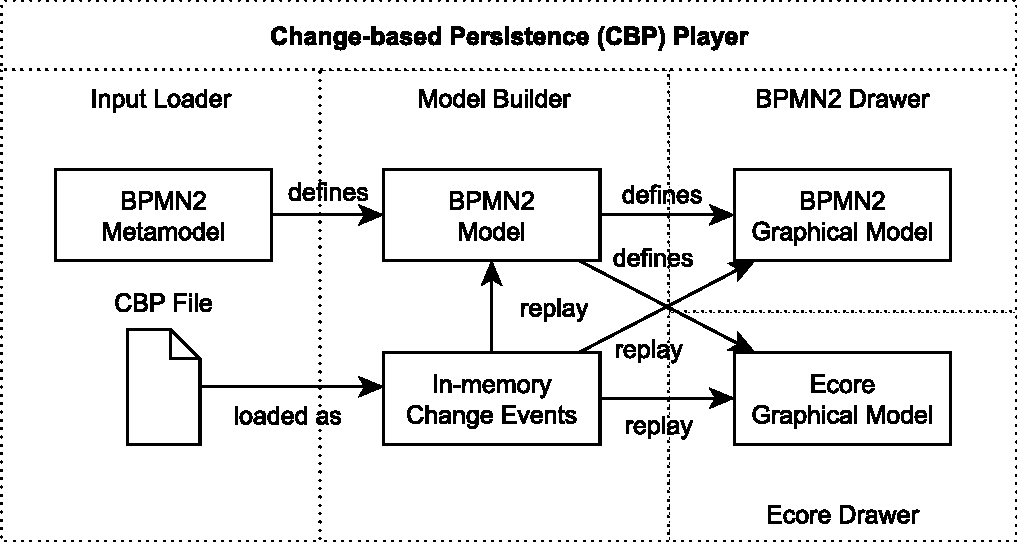
\includegraphics[width=\linewidth]{architecture}
    \caption{An architecture to visualise model construction using change-based persistence.}
    \label{fig:architecture}
\end{figure}

\subsection{Prototype}
\label{sec:prototype}

\begin{figure}[]
    \frame{\includegraphics[width=\linewidth]{prototype}}
    \caption{A simple application that visualise the construction of the model in Fig. \ref{fig:bpmn2} in two perspective:
        Ecore and BPMN2.}
    \label{fig:prototype}
\end{figure}

A simple application that visualises the construction of the model in Fig. \ref{fig:bpmn2} in two perspective,
Ecore and BPMN2, at the moment when edge \texttt{e3} is about to be removed (Lst. \ref{lst:bpmn2_cbp}, line 15).

\section{Evaluation}
\label{sec:evaluation}
We have not attempted performance evaluation for the work reported in this paper 
as the current version of the prototype is not intentionally not optimised for performance.


\section{Related Work}
\label{sec:related_work}

\section{Conclusions and Future Work}
\label{sec:conclusions_and_future_work}

\section*{Acknowledgment}
This work was partly supported by through a scholarship managed by \emph{Lembaga Pengelola Dana Pendidikan Indonesia} (Indonesia Endowment Fund for Education).

%\section*{References}
\bibliographystyle{IEEETran}
\bibliography{references}

\end{document}
